\chapter{Hidden Markov Models}
Hidden Markov Models are known to be used in various areas like speech recognition, biological sequence selection, piracy detection, and study of protein structure. In past few years, they are known to be used for detecting the metamorphic malware. The HMMs are trained by using the opcodes from known malware and then once the HMM has been trained, it can be used to score files [28].

\section{Overview of HMMs}
The Hidden Markov models (HMMs) are the state machine based statistical models which can be used to describe a set of observations generated by a stochastic process [24]. These processes can be demonstrated as state sequences, where the next state depends purely on the present state. Let us demonstrate the Hidden Markov Models using Dr. Stamp\rq s paper [25].

In an example from this paper, the problem is to determine the average annual temperature at a specific location over a period of time. Also, let us consider that there was no accurate way to determine the temperature during the period of time under question. As, there are no recorded past temperatures, we would consider only two annual temperature descriptions, one is \lq hot \rq and other is \lq cold\rq. Suppose, the scientists have arrived at probability of 0.6 for a cold year to be followed by a cold year, and \lq 0.7 \rq for a hot year that is followed by a hot year. This information can be denoted in the form of matrix as follows:

\begin{figure}[htb]
\centering
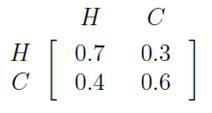
\includegraphics[width=0.3\textwidth]{images/mat.jpg}
\caption{Matrix for temperature probabilities} 
\label{fig:Matrix for temperature probabilities}
\end{figure}
\break

where H is hot and C is cold.
Also, we assume that the current research indicates a correlation between the size of tree growth rings and temperature [25]. For simplicity, let us consider three different rings, small (S), medium (M) and large (L). The probabilistic relationship between annual temperature and the tree ring sizes can be assumed to be as follows:
$$ \left[
  \begin{array}{c c c}
     0.1& 0.4& 0.5\\
     0.7& 0.2& 0.1
  \end{array} \right]
$$

For the above example, the state is the average annual temperature \textemdash H or C. The next state depends only on the current state, and hence the transition from one state to the next is a Markov process. We cannot directly have an access to the temperatures of the past, and so the actual states are known to be \lq hidden\rq. Although we cannot observe the temperature directly, we can still observe the tree ring sizes. Since, the states are hidden, the model is known as Hidden Markov model. 

The transition matrix will look as follows:
$$ A = \left[
  \begin{array}{c c}
     0.7& 0.3\\
     0.4& 0.6
  \end{array} \right]
$$
and 
$$ B = \left[
  \begin{array}{c c c}
     0.1 0.4 0.5\\
     0.7 0.2 0.1
  \end{array} \right]
$$

Let us suppose that the initial state distribution, denoted by $\pi$, is 
$\pi$ = [0.6 0.4]

All the matrices above are row stochastic, that is, all the elements of each row sum up to 1 and each element is a probability. Now, if we consider a four year period, for which we observe the series of the rings as S, M, S, L. Let S be 0, M be 1 and L be 2. Therefore, the observation sequence is 
O = (0, 1, 0, 2).

We might want to determine the most likely state sequence of the Markov process, given the above observations. That is, for the above example, we might want to know the most likely average annual temperature. We can reasonably define the most likely as the state sequence that exploits the expected number of correct states. We can use HMMs to find this sequence. We will now have a look at the notations, which are the most challenging part of HMM. The notations as described in [25] are as follows:\\
Let\\
T = length of the observation sequence\\
N = number of states in the model\\
M = number of observation symbols\\
Q = ${q_{0}, q_{1}, . . . , q_{N\textemdash1}}$ = distinct states of the Markov process\\
V = {0, 1, . . . , M\textemdash1} = set of possible observations\\
A = state transition probabilities\\
B = observation probability matrix\\
$\pi$ = initial state distribution\\
O = $(O_0, O_1,\dots, O_{T\textemdash1})$ = observation sequence.\\ 

\begin{figure}[htb]
\centering
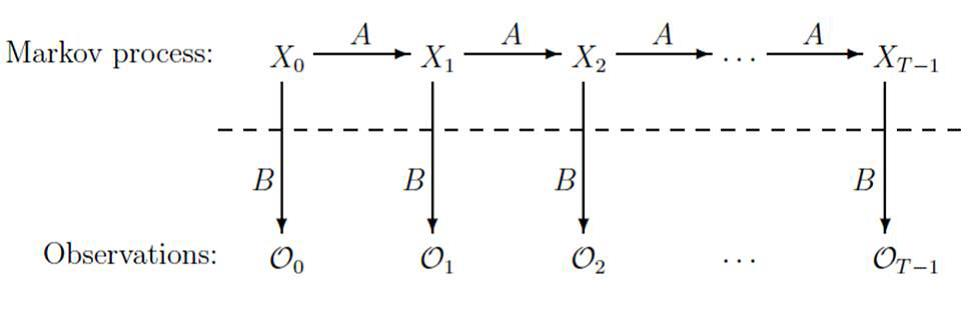
\includegraphics[width=0.8\textwidth]{images/markov.jpg}
\caption{Markov process} 
\label{fig:Markov process}
\end{figure}
\pagebreak
The above figure taken from [23] denotes a generic HMM.$ X_0 , X_1 , \dots, X_T $ denotes the hidden state sequence. The hidden Markov process is shown above the hidden line. The observations corresponding to the hidden states are connected by B. 

For the temperature example described above, we have T = 4, N = 2, M =3, Q = {H,C}, V ={0, 1, 2} where 0, 1, 2 represent the tree ring sizes. The Hidden Markov Model is defined by A, B and $\pi$. The HMM is denoted as $\lambda$ = (A, B, $\pi$). The HMM is denoted as $\lambda$ = (A, B, $\pi$).
Let us consider a state sequence of length four.
X =$(x_0, x_1, x_2, x_3)$ with corresponding observations O =$(O_0, O_1, O_2, O_3)$

Then $\pi x_0$ is the probability of starting in state $x_0$. Also, $b x_0$ $(O_0)$ is the probability of initially observing $O_0$ and $a x_0$, $x_1$ is the probability of transition from state $x_0$ to state $x_1$. Continuing, we see that the probability of the state sequence X is given by 
P(X) = $\pi x_0$ $b x_0$ $(O_0)$ $a x_0$, $ x_1$ $b x_1 (O_1)$ $a x_1$, $x_2$ $b x_2$ $(O_2) a x_2$,$x_3 b x_3(O_3)$.

With the example described above, we have the sequence O = (0, 1, 0, 2). We can compute the probability as follows:

P(H H C C ) = = 0.6(0.1)(0.7)(0.4)(0.3)(0.7)(0.6)(0.1) = 0.000212

In a similar way, the probability of each possible state can be calculated. To find the most probable sequence, we have to look at each position independently and find which of the two \lq H\rq or \lq C\rq have a higher probability for that particular position. We then choose the state having the higher probability for that position. We can add the normalized probabilities of all sequences starting with either H or C. The one with the higher probability best fits that position. The calculated probabilities for each position are given in the table below [23]:

\begin{figure}
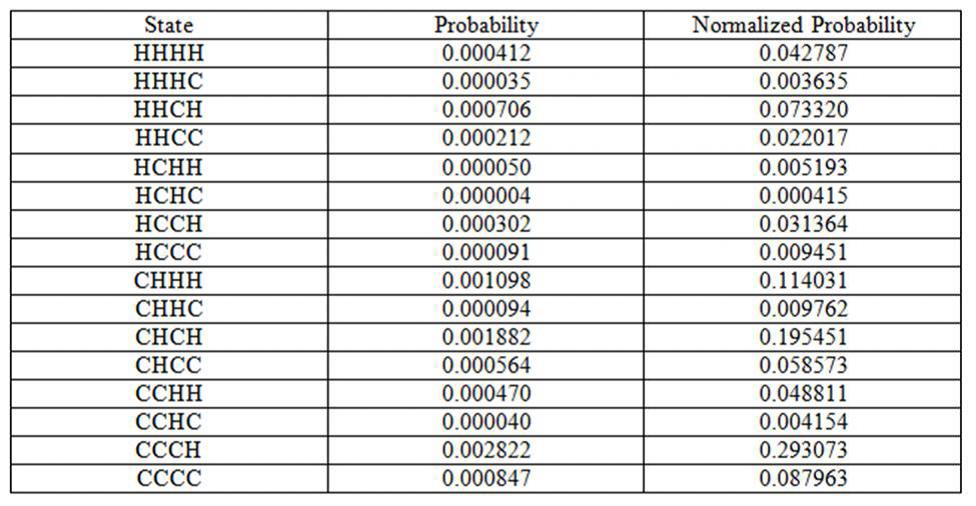
\includegraphics[width=1.0\textwidth]{images/prob.jpg}
\caption{Probabilities} 
\label{table:Probabilities}
\end{figure}
\break

Using the table below, we can now pick up the state with the highest probability.

\begin{figure}
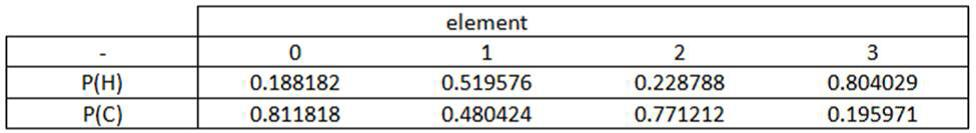
\includegraphics[width=0.7\textwidth]{images/prob2.jpg}
\caption{State with highest probabilities} 
\label{table: with highest probabilities}
\end{figure}
\break

The optimal sequence will be CHCH.

\section{Threshold Approach}
As described in Wong and Stamp\rq s paper, threshold approach [26] can be used for detecting the malware. The HMMs are first trained and then are used to detect malware. The working of the threshold model can be described as follows:
\begin{enumerate}
\item A single HMM can be trained using the known malware file opcode sequences.
\item This results can be observed by performing multiple runs to obtain a threshold value. Once, the threshold value is obtained, all the files scoring below the threshold can be classified as benign and ones scoring above as malicious.
\end{enumerate}

\section{Dueling Approach}
The dueling HMM strategy is used to address the challenges that are faced by threshold approach by introducing multiple HMMs. The dueling approach was developed in order to perform a more accurate analysis. The term dueling denotes that multiple HMMs compete with each other to decide which one is the best. 

The approach used by dueling HMM is as follows:
\begin{enumerate}
\item Train multiple HMMs, the number being same as the number of malware and benign files. This will result into an individual HMM for each uninfected as well as infected file. 
\item The file to be classified is scored against each of the HMM and the scores are recorded.
\item The file is classified as belonging to the HMM which scored the highest.
\end{enumerate}

The time required for the analysis is more as each file needs to be compared against multiple HMMs. The result for the dueling approach is improved as compared to the threshold approach. 